\subsubsection{Sprint goal}
L'obiettivo dello sprint è stato quello di concludere l'epica riguardante la visualizzazione e l'analisi dei tweet.\\
Nello specifico, sono state implementate le seguenti funzionalità:
\begin{itemize}
    \item Ricerca di tweet per intervallo temporale (richiesto dal cliente allo sprint review precedente)
    \item Ricerca di un determinato numero di tweet con una singola ricerca (richiesto dal cliente allo sprint review precedente)
    \item Ricerca di tweet per parola chiave
    \item Mappa per visualizzare la posizione dei tweet con geolocalizzazione
    \item Raccolta di tweet in tempo reale
\end{itemize}

\subsubsection{Backlog}
\userstory%
{Come utente,\\voglio scegliere un numero di tweet da poter caricare in una volta\\per poterli analizzare in modo aggregato.}%
{5\\(3 frontend + 2 backend)}%
{Possibilità di ricercare un largo numero di tweet scrivendone la quantità in un textbox. 
Tale quantità serve per la ricerca iniziale e anche per mostrare pagine successive. 
È possibile inoltre ricercare un numero di tweet inizialmente per poi cambiare quantità e cercare una pagina successiva 
(esempio: ricerca di 150 tweet iniziali, poi viene modificata la quantità (dallo stesso textbox) in 20 e si preme su “Pagina successiva”. Il numero di tweet così mostrato diventa 170).}%
{}

\userstory%
{Come utente,\\voglio scegliere un intervallo di tempo e raccogliere tweet\\per analizzarne le tendenze storiche.}%
{5\\(3 frontend + 2 backend)}%
{Possibilità di ricercare dei tweet dato un intervallo temporale. Non deve essere possibile cercare tweet nel futuro. 
Non deve essere possibile cliccare su “Prossima pagina” quando non ci sono più tweet da visualizzare.}%
{}

\userstory%
{Come utente interessato a vedere tweet,\\voglio poter cercare dei tweet per parola chiave\\per vedere cosa ne pensa la gente a riguardo.}%
{4\\(2 frontend + 2 backend)}%
{Possibilità di cercare tweet per parola o frase chiave. I grafici già presenti devono funzionare anche con questa ricerca.}%
{}

\userstory%
{Come utente interessato ai tweet,\\voglio poter visualizzare su una mappa la posizione dei tweet cercati\\per avere un'idea della località dalla quale sono stati pubblicati.}%
{7\\(3 frontend + 4 backend)}%
{Possibilità di visualizzare una mappa con le posizioni dei tweet ricercati. 
Se sono presenti più tweet nella stessa zona è possibile aggregarli (in base alla distanza) e mostrare un unico valore, 
ovvero il numero di tweet in tale zona. La mappa deve essere sempre visibile anche durante lo scorrimento della pagina (come i grafici).}%
{}

\userstory%
{Come utente,\\voglio vedere la posizione di tutti i tweet di una data persona\\per conoscere i suoi spostamenti.}%
{5\\(5 frontend + 0 backend)}%
{Possibilità di inserire il nome utente di una persona e visualizzare su una mappa le posizioni dei suoi tweet e i suoi spostamenti. 
Per gli spostamenti si mostrano sulla mappa delle frecce basandosi sulla posizione e sulla data del tweet.}%
{}

\userstory%
{Come lettore di tweet,\\voglio poter vedere i tweet che ricerco in tempo reale\\per sapere cosa la gente posta.}%
{10\\(3 frontend + 7 backend)}%
{}%
{}


\subsubsection{Burndown}
\begin{figure}[H]
    \centering
    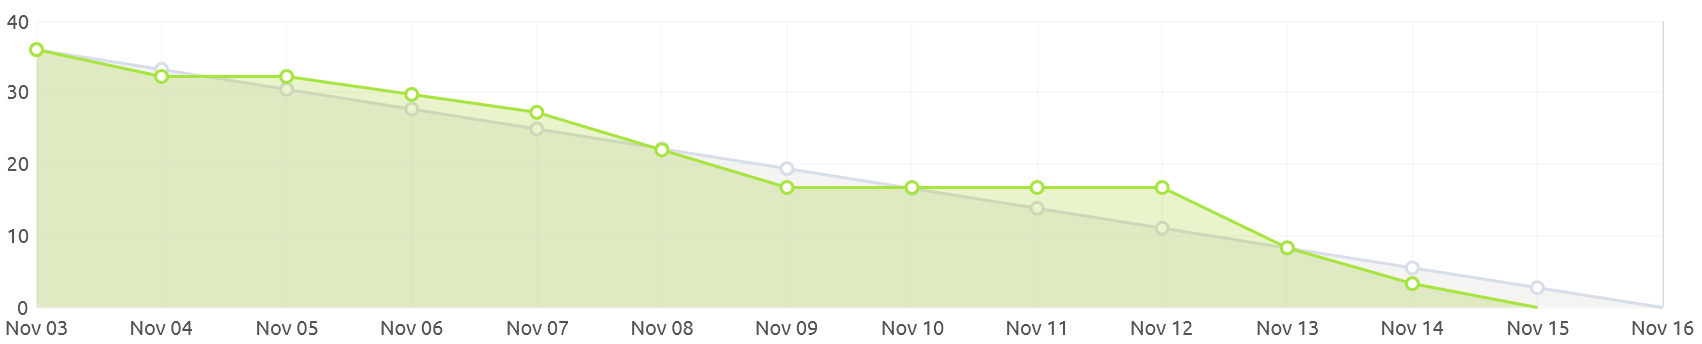
\includegraphics[width=15cm]{./img/sprint2/burndown.png}
    \caption{Burndown}
\end{figure}
\begin{figure}[H]
    \centering
    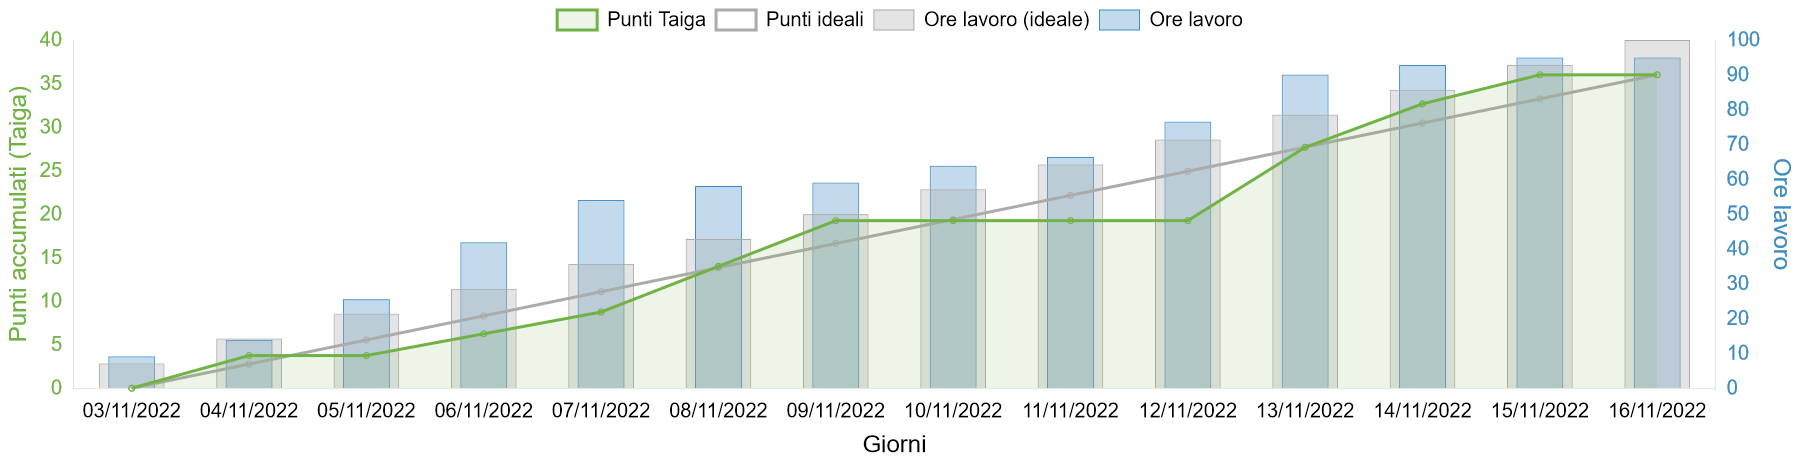
\includegraphics[width=15cm]{./img/sprint2/worktime.png}
    \caption{Progresso dei punti (asse a sinistra) e ore di lavoro (asse a destra)}
\end{figure}

\subsubsection{Retrospettiva}
\begin{figure}[H]
    \centering
    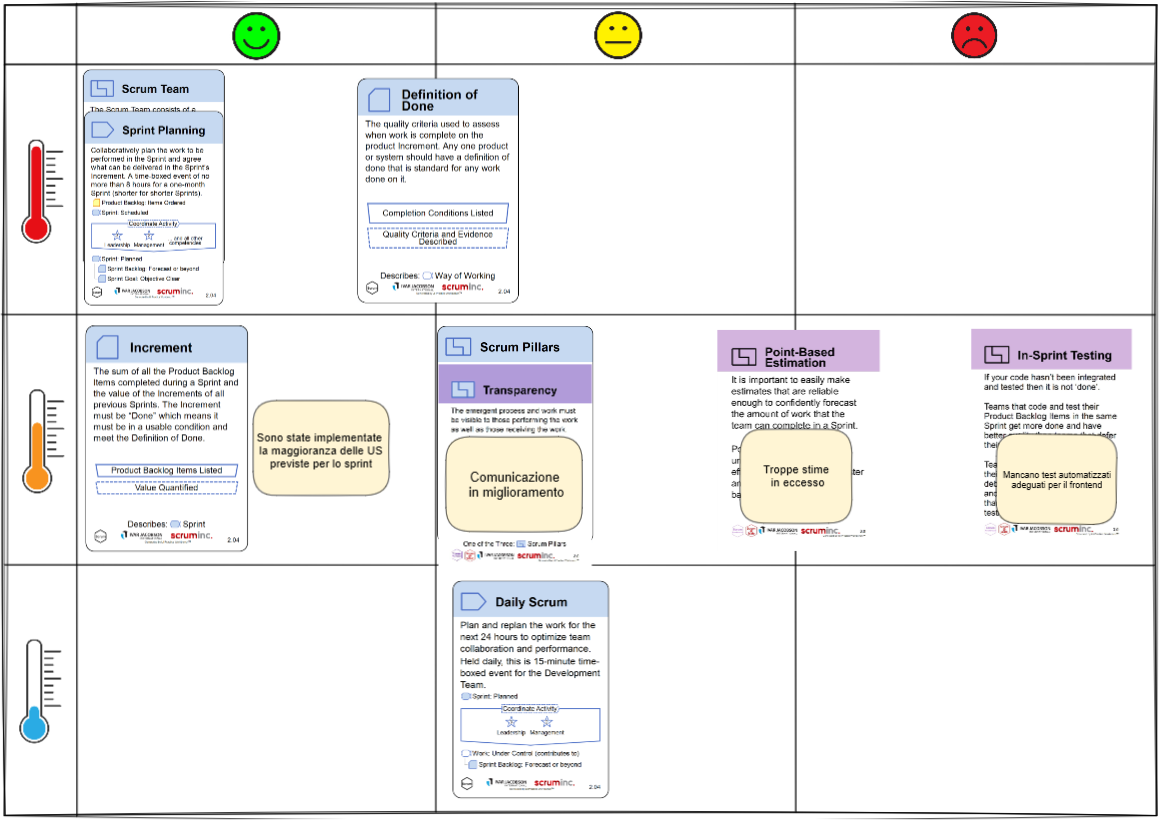
\includegraphics[width=15cm]{./img/sprint2/preretrospettiva.png}
    \caption{Pre-retrospettiva del 10/11/2022}
\end{figure}